\documentclass[12pt]{article}
\usepackage{amsmath, amssymb}
\usepackage{geometry}
\geometry{a4paper, margin=1in}
\usepackage{parskip}
\usepackage{graphicx}
\usepackage{tikz}
\usepackage{pgfplots}
\pgfplotsset{compat=1.18}
\usetikzlibrary{shapes.geometric, arrows.meta, positioning}
\usepackage{enumitem}
\usepackage{xcolor}
\usepackage{listings}
\usepackage{booktabs}
\usepackage{hyperref}
\hypersetup{colorlinks=true, linkcolor=blue!60!black, citecolor=blue!60!black, urlcolor=blue!60!black}

\lstdefinelanguage{JavaScriptRSVP}{
  keywords={function, const, let, var, if, else, for, while, return, new, this, Math, Float32Array, JSON, localStorage, performance, Date},
  keywordstyle=\color{blue!60!black}\bfseries,
  comment=[l]{//},
  commentstyle=\color{gray}\itshape,
  string=[b]",
  stringstyle=\color{orange!70!black},
  basicstyle=\ttfamily\footnotesize,
  breaklines=true,
  showstringspaces=false,
  numbers=left,
  numberstyle=\tiny\color{gray},
  frame=single,
  tabsize=2
}

\title{A Relativistic Theory of Longevity}
\author{Flyxion}
\date{August 2026}

\begin{document}
\maketitle

\begin{abstract}
This essay reconceives longevity as a special case of a more general condition: the recoverability of a distinction under transformation. Rather than beginning from a field-theoretic picture of the organism, it begins from the minimal apparatus of a structured domain --- a space of states, a family of transformations that degrade them, and a family of admissible reconstruction operators capable of restoring what those transformations threaten to destroy. An organism, on this view, is not a fixed material configuration but a \emph{persistence attractor}: a pattern of distinctions that remains recoverable, and therefore identifiable as the same organism, across continuous replacement of its substrate. Longevity is the maintained sufficiency of an organism's repair operators against the transformations that erode it; aging is what happens when that sufficiency fails.

Biologically, this principle is given a concrete architecture in the Hepastitium: a distributed program of continuous tomographic sensing coupled to enormous numbers of small, targeted repair interventions, converting medicine from episodic diagnosis into endogenous maintenance. A working precursor to this architecture already exists in Physiome, the author's Rust-based whole-body physiology simulator, whose eleven interacting organ systems are governed by admissibility and repair operators rather than fixed differential equations --- the diagnostic and homeostatic half of the Hepastitium's program, already running. The same repair-theoretic vocabulary extends to architecture, where xylomorphic cities are treated as distributed reconstruction systems; to epistemics, where a semantic microscope organizes medical knowledge around recoverable causal structure rather than disease taxonomy, disciplined by an explicit Record-Recognize-Interpret-Admit-Intervene-Verify pipeline that keeps detection from collapsing directly into intervention; to cognition, where longevity means the continuity of a self-reconstructing cognitive frame under transformation, informed both by a relativistic account of consciousness and by the general theory of self-reconstruction as a persistence attractor; and to the longevity of a lineage, where the classical grandparent hypothesis and the reallocation of cognitive resources in old age are read as a shift from individual repair capacity toward distributed epistemic revisability at the level of the group.

A compact field-theoretic gloss of this material, in the author's earlier Relativistic Scalar-Vector Plenum (RSVP) notation, is retained as an optional appendix for readers who want it; nothing in the main argument depends on it.

\medskip
\noindent \textbf{Keywords:} recoverable distinction; persistence; repair operators; Hepastitium; Physiome; admissibility; cognitive anti-senescence; distributed reconstruction.
\end{abstract}

\section{Introduction}

The quest for longevity has historically been framed as a battle against entropy, drawing on thermodynamic principles articulated by Clausius and Boltzmann, and later reframed by Prigogine's dissipative structures, which emphasized self-organization in far-from-equilibrium systems \cite{prigogine1977}. Schr\"odinger's seminal question, ``What is Life?'', posited life as a negentropic process, extracting order from environmental chaos \cite{schrodinger1944}. Contemporary longevity paradigms---genetic engineering, cellular therapies, cryonics, or AI consciousness uploads---often resist entropy through localized interventions, failing to address systemic recursion across scales.

This essay takes a different starting point than an earlier version of this argument, which built its formalism directly on a field-theoretic picture of the organism. Here the more general apparatus comes first: a structured domain consisting of a state space, a family of transformations that act upon it, a family of distinctions that can be drawn within it, and a family of reconstruction operators capable of recovering those distinctions after transformation \cite{flyxion2026persistence}. Longevity is then a claim about the second and fourth of these components --- about whether reconstruction remains sufficient against transformation --- rather than a claim about any particular substrate, field, or set of coupled equations. This reframing is not merely terminological. It clarifies what earlier language obscured: that the relevant question for an organism, an institution, or a mind is never whether its material composition stays fixed, but whether the distinctions that make it \emph{that} organism, institution, or mind remain recoverable as the composition changes.

Section~\ref{sec:persistence} develops this minimal apparatus and states the resulting persistence criterion for organisms. Section~\ref{sec:hepastitium} applies it biologically through the Hepastitium, and introduces Physiome, the author's working physiology simulator, as a concrete present-day instantiation of its diagnostic and homeostatic half. Section~\ref{sec:architecture} extends the same apparatus to architecture and civilizational infrastructure. Section~\ref{sec:allostasis} supplies the epistemic discipline that keeps detected deviations from triggering intervention automatically. Section~\ref{sec:cognitive} extends the persistence criterion to cognition, where the hardest form of the continuity question arises. Section~\ref{sec:lineage} extends it once more, to longevity distributed across a lineage rather than sustained within a single organism. A field-theoretic restatement of the core formalism, in the author's earlier Relativistic Scalar-Vector Plenum (RSVP) notation, is given as an optional appendix.

\label{sec:intro}

\section{Recoverable Distinction and the Persistence of Organisms}
\label{sec:persistence}

The framework used throughout this essay is deliberately minimal. Let
\[
\mathfrak{D} = (X, \mathcal{T}, \mathcal{D}, \mathcal{R})
\]
be a structured domain: a state space $X$, a family of admissible transformations $\mathcal{T} = \{T_\alpha : X \to X\}$, a family of distinctions $\mathcal{D} = \{d_i : X \to Y_i\}$ that can be drawn on $X$, and a family of reconstruction operators $\mathcal{R} = \{R_j : X \to X\}$ capable of restoring distinctions after transformation \cite{flyxion2026persistence}. For an organism, $X$ is the space of physiologically reachable tissue and cellular configurations; $\mathcal{T}$ is the set of transformations that degrade it --- ordinary metabolic damage, injury, mutation, replicative error, environmental insult; $\mathcal{D}$ is the family of functional and structural distinctions that matter to the organism's identity and viability; and $\mathcal{R}$ is the family of repair, replacement, and regenerative processes available to it, biological or engineered.

A distinction $d$ is \emph{recoverably persistent} under a transformation $T$ if there exists a reconstruction operator $R \in \mathcal{R}$ such that
\begin{equation}
d \circ R \circ T = d.
\label{eq:recoverable-persistence}
\end{equation}
This condition is strictly weaker than classical invariance ($d \circ T = d$, recovered as the special case $R = \mathrm{id}$), and this generalization is the entire point: almost nothing about a living organism is literally invariant under the transformations acting on it from moment to moment. Cells die and are replaced. Proteins misfold and are degraded. What persists is not the material substrate but the recoverability of the distinctions that matter --- a claim about repair, not about preservation.

\subsection{Repair Operators and the Persistence Potential}

Following the same framework, define the persistence potential of a distinction $d$ as the expected reconstruction error the distinction would incur under the transformations it is likely to face,
\begin{equation}
\Phi(d) = \bar{P}(d) = \int_{\mathcal{T}} P(d,T)\, d\mu(T), \qquad P(d,T) = \inf_{R \in \mathcal{R}} \Delta(d,T,R),
\label{eq:persistence-potential}
\end{equation}
where $\Delta(d,T,R)$ measures the residual discrepancy between $d$ and its reconstruction after $T$ and $R$ have acted, and $\mu$ is a measure over the transformation family reflecting how often each kind of damage actually occurs. Low $\Phi(d)$ means the distinction is robust: damage to it can be reliably reversed. High $\Phi(d)$ means the distinction is fragile.

A \emph{repair operator} is then any map $\rho : \mathcal{D} \to \mathcal{D}$ satisfying
\begin{equation}
\Phi(\rho(d)) \le \Phi(d).
\label{eq:repair-operator}
\end{equation}
A repair operator never increases persistence potential; it may leave it unchanged (no useful repair occurred) or decrease it (damage was successfully reversed). Repair operators compose: if $\rho_1$ and $\rho_2$ are repair operators, so is $\rho_2 \circ \rho_1$, since $\Phi(\rho_2(\rho_1(d))) \le \Phi(\rho_1(d)) \le \Phi(d)$ \cite{flyxion2026persistence}. This closure result is doing real work here: it is exactly what licenses treating a layered biological repair architecture --- DNA repair, protein quality control, immune clearance, and eventually the distributed microsurgery of Section~\ref{sec:hepastitium} --- as a single coherent maintenance system rather than an ad hoc collection of unrelated mechanisms. Each layer is a repair operator; their composition, by the closure property, is also a repair operator, whatever its internal complexity.

\subsection{The Longevity Condition}

An organism's viability over an interval requires that its repair regime, taken as a whole, keep its persistence potential from drifting upward on average. Writing $d_t$ for the organism's relevant distinctions at time $t$, $T_t$ for the damage-producing transformations acting between $t$ and $t+1$, and $\rho_t$ for the repair operator applied in response, the longevity condition is
\begin{equation}
\mathbb{E}\big[\Phi(\rho_t(T_t(d_t))) - \Phi(d_t)\big] \le 0.
\label{eq:longevity-condition}
\end{equation}
This is a direct descendant of the informal claim that repair must keep pace with damage, made precise: it says nothing about any specific field or substrate, only that the organism's own reconstruction operators must, on average, not lose ground against the transformations degrading it. Equation~\eqref{eq:longevity-condition} is the criterion this essay will apply, in progressively more concrete form, to tissue (Section~\ref{sec:hepastitium}), to cognition (Section~\ref{sec:cognitive}), and to the lineage as a whole (Section~\ref{sec:lineage}).

\subsection{Identity as a Persistence Attractor}

A further consequence of this framework matters more than it may first appear. Objects, on this account, are not primitive; they are equivalence classes of states that repeated reconstruction converges toward --- \emph{persistence attractors} \cite{flyxion2026persistence}. An organism's identity is not carried by any fixed collection of atoms, cells, or even organs. It is carried by the fact that reconstruction, applied again and again across metabolic turnover, injury, and repair, keeps returning to the same recognizable pattern of distinctions. This reframing does real work later in the essay (Section~\ref{sec:ethics}, Section~\ref{sec:cognitive}): it is what allows morphological change, tissue replacement, and even substrate transition to be evaluated by a single consistent criterion --- does reconstruction still converge to the same attractor? --- rather than by an intuition about material continuity that biology has never actually satisfied.

\subsection{Repair as an Operational Process}

The longevity condition of Equation~\eqref{eq:longevity-condition} can be given a more operational, step-by-step form. Writing $x_t \in X$ for the organism's state at time $t$, $D_t$ for the disturbance operator acting between $t$ and $t+1$ (damage, injury, ordinary metabolic wear), and $R_t$ for the repair repertoire actually available at that moment, a single maintenance cycle is
\begin{equation}
x_{t+1} = R_t\big(D_t(x_t)\big), \qquad x_{t+1} \in \mathcal{A},
\label{eq:repair-cycle}
\end{equation}
where $\mathcal{A} \subset X$ is the admissible set: the region of state space within which the organism's identity-defining distinctions remain recoverable in the sense of Equation~\eqref{eq:recoverable-persistence}. Equation~\eqref{eq:longevity-condition} is the statement that, on average, this cycle keeps landing back in $\mathcal{A}$; Equation~\eqref{eq:repair-cycle} is what that landing looks like on any given day.

\subsection{Aging as Contraction of the Recoverable Region}
\label{sec:recoverable-region}

This operational form suggests a sharper account of aging than a bare rise in persistence potential. Let $\mathcal{R}_t \subseteq X$ denote the \emph{recoverable region} around the organism's current state at time $t$: the set of disturbances from which some available $R_t$ can still return the system to $\mathcal{A}$ within bounded time and bounded residual damage. Aging, on this account, is the tendency of that region to contract:
\begin{equation}
\mathcal{R}_{t+1} \subseteq \mathcal{R}_t.
\label{eq:recoverable-contraction}
\end{equation}
This is a stronger and more specific claim than ``damage accumulates.'' Two organisms can occupy very similar observable states at a given moment while having sharply different $\mathcal{R}_t$: one can still absorb a large infection, a bone fracture, or a week of sleep deprivation and return to $\mathcal{A}$; the other, superficially similar, cannot. Chronological age is a poor proxy for this quantity precisely because it measures elapsed time rather than the shape of $\mathcal{R}_t$ itself. This also sharpens what rejuvenation would have to mean on this framework: not restoring $x_t$ to resemble some earlier snapshot $x_{t_0}$, but enlarging $\mathcal{R}_t$ --- widening the set of futures from which the organism can still recover, whatever its current state happens to look like.

This reframing yields the essay's central claim in its most compact form:
\begin{equation}
\boxed{\text{Aging is not the accumulation of time. It is the progressive loss of recoverable futures.}}
\label{eq:aging-thesis}
\end{equation}
It is worth being explicit about why this formulation is preferred over a cruder one built directly on an entropy-like quantity that simply counts disorder or elapsed change. A system undergoing no dynamics at all, a system undergoing purely random dynamics, and a system undergoing perfectly reversible dynamics can all present the same superficial profile to a naively defined disorder measure, because such a measure does not distinguish a trajectory that has genuinely foreclosed future reconstruction from one that merely looks different at successive instants. What actually matters, and what Equation~\eqref{eq:recoverable-contraction} is built to track directly, is the loss of reconstructible trajectories, not a raw count of change or disorder --- a distinction developed at greater length, independently of longevity, elsewhere in the author's work on irreversibility \cite{flyxion2026worldhood}. Grounding aging in $\mathcal{R}_t$ rather than in a bare entropy term avoids quietly reintroducing elapsed time as a hidden clock inside a theory whose entire point is that biological age is not clock time.

\section{Physiome: A Measurement and Modeling Layer for Recoverability}
\label{sec:physiome}

The framework of Section~\ref{sec:persistence} specifies what persistence means for an organism. It does not, by itself, specify what can actually be measured or modeled to test it. That is the role of \emph{Physiome}, the author's whole-body physiology simulator, introduced at this point in the essay precisely because it is the bridge between the ontology just developed and the biological application that follows.

Physiome is a whole-body physiology simulator written in Rust and built around admissibility and repair operators rather than a fixed system of ordinary differential equations. It implements eleven interacting organ systems --- cardiovascular, renal, hepatic, gastrointestinal, autonomic and central nervous, immune, hematologic and coagulation, endocrine, metabolic, respiratory, and thermal --- each represented as a structured domain in the sense of Section~\ref{sec:persistence}, with homeostatic correction governed by admissibility constraints and repair operators local to each subsystem. Concretely, Physiome is machinery for asking which physiological distinctions actually remain reconstructible across scales --- electrical, mechanical, metabolic, circulatory, endocrine, cellular, and organ-level --- rather than a further theory of what an organism ``really is.'' Section~\ref{sec:persistence} says what persistence means; Physiome says what can be measured and modeled to test it. That separation is deliberate, and it is what licenses returning to Physiome a second time, in Section~\ref{sec:empirical}, with actual candidate measurements rather than a restatement of the same claim.

Physiome is deliberately the smaller, more honest claim next to the Hepastitium's larger speculative one, introduced in Section~\ref{sec:hepastitium}: it does not perform microsurgery, and it does not remodel morphology. What it does do is demonstrate, in working code with a worked multi-hour infection scenario and a passing test suite, that the admissibility-and-repair framework of Section~\ref{sec:persistence} is not merely a redescription of ordinary physiological modeling but an actually implementable alternative to it --- one in which homeostatic correction is represented explicitly as the repair operators of Equation~\eqref{eq:repair-operator}, coupled across subsystems, rather than smuggled into the coefficients of a fixed equation. As such, Physiome functions as the present-day empirical and computational anchor for the entire framework of this essay: every claim made abstractly in Section~\ref{sec:persistence} about repair operators, persistence potential, recoverable regions, and closure under composition is, for eleven organ systems at least, something that already runs.

\section{Biological Longevity: The Hepastitium}
\label{sec:hepastitium}

The Hepastitium, derived from Greek \emph{hepar} (liver) and Latin \emph{stitium} (standing-place or structure), denotes an endogenous, distributed network for continuous tissue maintenance. It extends the regenerative role of the liver to every organ system, transforming the entire organism into a coordinated repair architecture. Within the framework of Section~\ref{sec:persistence}, the Hepastitium operationalizes longevity as the practical satisfaction of Equation~\eqref{eq:longevity-condition}: the capacity to keep persistence potential from drifting upward through distributed sensing and distributed microsurgical repair.

\subsection{Mechanisms}

The Hepastitium integrates hardware, software, and informational layers into a coherent recursive feedback network:

\begin{itemize}[leftmargin=*]
\item \textbf{Tomographic Relays:} Low-intensity X-ray, ultrasound, and terahertz arrays provide noninvasive, full-body imaging at cellular resolution. Each voxel is mapped to a local estimate of persistence potential, producing a continuously updated four-dimensional map of where distinctions are fragile. Reconstruction pipelines employ compressive sensing and Bayesian inference to minimize radiation exposure while maintaining spatial precision. These relays constitute the \emph{Record} and \emph{Recognize} stages of the pipeline formalized in Section~\ref{sec:allostasis}: they generate candidate distinctions and flag anomalous patterns without themselves authorizing any response.

\item \textbf{Microsurgical Robots:} Millions of sub-millimeter endothelial agents operate within the vascular system, guided by the persistence-potential map. Each robot executes targeted interventions such as plaque clearance, synaptic modulation, or DNA repair. Each such intervention is a repair operator in the sense of Equation~\eqref{eq:repair-operator}, and the network's coordination emerges through the shared objective of driving the aggregate longevity condition, Equation~\eqref{eq:longevity-condition}, toward satisfaction rather than through any centralized control scheme.

\item \textbf{Morphological Agency:} The same microsurgical infrastructure enables macroscopic, reversible transformations---height modulation through osteogenic scaffold elongation, limb reshaping via perfusion control, or body resizing through temporary metabolic reprogramming. Section~\ref{sec:persistence} makes clear what licenses this: such changes are admissible exactly when the organism's persistence attractor --- its recoverable identity --- survives the transformation, so that morphology becomes a parameter of ongoing reconstruction rather than a fixed constraint.
\end{itemize}

Together, these components transform medicine from a reactive intervention to a continuous discipline of reconstruction. The Hepastitium maintains viability by sustaining the body as a distributed, self-observing system engaged in ongoing repair.

\subsection{Evolutionary Analogy}

The Hepastitium constitutes an evolutionary threshold: a transition from stochastic cellular maintenance to deliberate, coordinated repair. Natural biology relies on probabilistic micro-repairs---apoptosis, autophagy, immune pruning---where each event occurs locally and blindly, guided by statistical survival rather than global coherence. In contrast, the Hepastitium implements a deterministic feedback system informed by a global map of persistence potential. This parallels the shift from Darwinian selection to Lamarckian adaptation: a movement from passive fitness filtering to active structural learning.

From an evolutionary thermodynamic perspective, the Hepastitium extends the logic of endosymbiosis---where mitochondria internalized energy production---into the realm of repair and regulation. The organism internalizes its own maintenance infrastructure, and the closure property of repair operators established in Section~\ref{sec:persistence} is precisely what licenses treating this internalized infrastructure, however many distinct mechanisms it comprises, as a single coherent repair regime.

\subsection{Energetic and Informational Constraints}

To remain physiologically viable, the Hepastitium must satisfy strict energy and information budgets. If each microsurgical event consumes energy $\epsilon_i$ and reduces persistence potential by $\Delta\Phi_i$, the daily balance condition is:
\begin{equation}
\sum_i \epsilon_i \le E_{\text{budget}}, \qquad \sum_i (-\Delta\Phi_i) \ge \eta_{\text{target}},
\label{eq:energy-budget}
\end{equation}
where $E_{\text{budget}}$ denotes total metabolic energy available for maintenance and $\eta_{\text{target}}$ defines the desired rate of persistence-potential reduction. This ensures that hepatic operations remain energy-neutral at the organismal scale. Information throughput is bounded by a recursive Shannon limit:
\begin{equation}
I_{\max} = \frac{E_{\text{budget}}}{k_B T \ln 2},
\label{eq:shannon-limit}
\end{equation}
linking thermodynamic efficiency to informational capacity and defining a quantitative ceiling for daily microsurgical data exchange.

\subsection{Energy Economics}

Continuous microsurgical operation within the Hepastitium demands a stable energetic substrate. Preliminary modeling suggests that maintaining millions of microsurgeries per day would consume approximately 10--20\% of the basal metabolic rate, depending on the efficiency of robotic circulation and data processing. Such a load is sustainable only if the energetic cost of intervention is offset by a proportional reduction in persistence potential across the tissues it acts upon.

The effective efficiency of the Hepastitium can be expressed as
\begin{equation}
\eta_{\text{eff}} = \frac{\sum_i (-\Delta\Phi_i)}{\sum_i \epsilon_i / (k_B T)},
\label{eq:efficiency}
\end{equation}
representing the persistence-potential reduction achieved per thermodynamic bit of energy expended. Effort is naturally allocated according to the local gradient of persistence potential, favoring regions of high fragility with high repair leverage --- the biological analogue of the persistence-descent dynamics described more generally elsewhere \cite{flyxion2026persistence}. In this sense the Hepastitium performs a thermodynamic arbitrage: it converts ATP expenditure into recoverable structure.

\subsection{Knowledge Infrastructure}

Medical knowledge under the Hepastitium paradigm must be reorganized around recoverable causal structure rather than static disease taxonomies. Instead of categorizing by pathology (what is wrong), the new epistemic architecture categorizes by reconstructive function (how a deviation propagates or is repaired). This transforms medicine into a recursive, explorable information system --- what this essay will continue to call the \emph{semantic microscope} --- governed by feedback loops and causal inference, and disciplined by the pipeline formalized in Section~\ref{sec:allostasis}.

Let $\mathcal{G} = (V, E)$ denote the medical knowledge graph. Each node $v_i \in V$ corresponds to a measurable distinction or repair operator, and each edge $e_{ij} \in E$ encodes a causal relationship with weight $w_{ij}$ proportional to observed repair efficiency. The graph evolves through continuous learning as new data from tomographic relays and microsurgical outcomes modify edge weights according to observed changes in persistence potential.

\begin{lstlisting}[language=JavaScriptRSVP, caption={Recursive update cycle of the semantic microscope.}, label={lst:update-graph}]
function updateGraph(G, delta_Phi):
    for node in G.nodes:
        if node.type == "distinction" and node.phi_estimate > Phi_c:
            for edge in G.edges(node):
                edge.weight += computeCausalInference(delta_Phi, edge)
    return G
\end{lstlisting}

Practically, this allows medical exploration through recursive queries such as identifying all procedures with a favorable ratio of persistence-potential reduction to energy cost, tracing causal chains reducing fragility in cardiac tissue by a target margin, or predicting emergent regions of fragility by extrapolating the persistence-potential map along high-weight edges.

\subsection{Allostasis, Admissibility, and the Epistemology of Repair}
\label{sec:allostasis}

The longevity condition of Equation~\eqref{eq:longevity-condition} is necessary but insufficient as a theory of intelligent maintenance. A system can efficiently drive persistence potential downward for some chosen distinction while catastrophically misunderstanding what should be preserved. The Hepastitium therefore needs an epistemic companion to its repair mechanics: a discipline governing when a measurement warrants an interpretation, and when an interpretation warrants an intervention.

The difficulty is that bodily measurements are not self-interpreting. A high heart rate, a cortisol change, an inflammatory marker, or an altered perfusion pattern cannot be assigned a fixed pathological or benign meaning independently of the organism's ongoing activity and history. Contemporary theories of constructed emotion make the same point about affect: the brain continuously predicts bodily needs and interprets ambiguous interoceptive signal against those predictions, rather than reading a raw, context-free measurement off the body \cite{barrettmiller2026longevity}. This is a special case of a more general regulatory principle known as allostasis, in which physiological set points are not fixed targets to be restored but variables that are adjusted in anticipation of predicted demand \cite{sterling2012}. If the organism's own regulatory apparatus already works this way, a hepatic operator that compares every tomographic reading against a single static reference body is not a refinement of biological regulation---it is a regression from it.

This motivates extending the distinctions that the semantic microscope tracks. Rather than a bare distinction $d_t$, the microscope should track a distinction together with its context and its anticipated continuation:
\begin{equation}
\hat{d}_t = (d_t, C_t, \Pi_{t:t+\tau}),
\label{eq:extended-distinction}
\end{equation}
where $C_t$ represents contextual information (recent activity, environmental load, circadian phase, and so forth) and $\Pi_{t:t+\tau}$ represents the predicted demands the organism is preparing to meet over some future interval $\tau$. The question the Hepastitium must answer is no longer simply whether a measurement departs from a population norm. It is whether the current configuration is appropriate for the continuation the organism is about to undertake.

To keep this predictive latitude from collapsing into unaccountable discretion, every candidate intervention must pass through an explicit pipeline rather than proceeding directly from detection to correction:
\begin{equation}
\text{Record} \;\rightarrow\; \text{Recognize} \;\rightarrow\; \text{Interpret} \;\rightarrow\; \text{Admit} \;\rightarrow\; \text{Intervene} \;\rightarrow\; \text{Verify}.
\label{eq:rraiv}
\end{equation}
A tomographic relay \emph{records} a tissue difference without thereby establishing that it is pathological. A classifier \emph{recognizes} a pattern in the recorded difference without proving its causal significance. The semantic microscope \emph{interprets} the recognized pattern against context and predicted demand, proposing but not yet authorizing a reading. \emph{Admission} means that the accumulated evidence---recorded, recognized, and interpreted---has crossed whatever threshold warrants intervention; this is a distinct step from interpretation itself, and a system that collapses the two treats every plausible story about a measurement as grounds for surgery. \emph{Intervention} is the microsurgical repair operator proper, of Equation~\eqref{eq:repair-operator}. \emph{Verification} closes the loop by determining, after the fact, whether the intervention actually reduced persistence potential as intended, rather than simply logging that an intervention occurred.

This pipeline also supplies a needed corrective to the optimization framing implicit elsewhere in this section. There is frequently no single scalar quantity that the Hepastitium should be maximizing. One intervention may improve cardiovascular reserve while degrading immune robustness; another may preserve cognitive throughput at greater basal energetic cost. The admissible region is therefore better modeled as a partially ordered set of continuations rather than a totally ordered scale with a unique maximum:
\begin{equation}
X_A \nprec X_B, \qquad X_B \nprec X_A, \qquad X_A, X_B \in \mathcal{A},
\label{eq:partial-order}
\end{equation}
where $\mathcal{A}$ is the admissible set defined by Equation~\eqref{eq:longevity-condition} together with the extended-distinction constraints of Equation~\eqref{eq:extended-distinction}. On this view the Hepastitium does not discover the one objectively correct body and drive the organism toward it; it identifies a region of jointly viable continuations and leaves the selection among them to the organism's own agency.

A further hazard belongs here precisely because the architecture is recursive. If the semantic microscope repeatedly interprets some benign variation as damage, intervenes against it, and then treats the resulting altered state as confirming evidence for the original interpretation, it can manufacture the very pathology it believes itself to be correcting---the biomedical analogue of a rigid affective category that reinforces itself through repeated misclassification. Guarding against this requires that the causal graph $\mathcal{G}$ of the preceding section retain more than confirmed successes: it must also preserve failed predictions, rejected interpretations, live counterfactual alternatives, and interventions that were deliberately withheld pending further evidence.

Together these considerations sharpen the persistence criterion of Equation~\eqref{eq:longevity-condition} into something with three distinguishable components rather than one:
\begin{equation}
\text{Longevity} \;=\; \text{repair capacity} \;+\; \text{epistemic revisability} \;+\; \text{continuation diversity}.
\label{eq:longevity-decomposition}
\end{equation}
A repair regime that efficiently reduces persistence potential but cannot revise its own interpretations, or that collapses a genuinely plural space of viable continuations into a single enforced target, satisfies the letter of Equation~\eqref{eq:longevity-condition} while failing the broader project this essay is concerned with. Section~\ref{sec:lineage} returns to this decomposition and argues that its second and third terms are, at the scale of a lineage rather than an individual, what aging itself is partly \emph{for}.

\subsection{Ethical Reflection}
\label{sec:ethics}

Morphological adaptations---including height modulation, body resizing, or organ-level reconfiguration---introduce profound ethical questions regarding identity, autonomy, and continuity. Section~\ref{sec:persistence} already supplies the relevant criterion: identity is not a function of material constancy but of whether reconstruction continues to converge on the same persistence attractor. If the distinctions that constitute the organism's self-model remain recoverable across a transformation, the organism---biological or cognitive---maintains its identity even as its morphology changes.

The Hepastitium therefore serves as both a biomedical and an ethical architecture. By anchoring all transformations within the recoverability condition of Equation~\eqref{eq:recoverable-persistence}, it guarantees that any morphological change respects the continuity of the organism's defining distinctions. In practical terms, this means that agency over form must be exercised through reversible, low-persistence-cost operations, ensuring that the individual's causal continuity---their experiential thread---remains unbroken across configurations.

Autonomy, in this context, is redefined as the freedom to transform without leaving the reconstruction pathway that defines one's own persistence attractor. The right to self-modification thus coexists with a responsibility to remain recoverable: a bioethical equilibrium between plasticity and persistence. This reversibility criterion replaces the older dichotomy of ``natural versus artificial'' with a gradient of recoverability---any transformation is permissible so long as the organism's identity-defining distinctions remain reconstructible across it.

At the societal level, the same principle extends to questions of enhancement, replication, and continuity across substrates. Cloning, uploading, or distributed embodiment may all preserve moral and personal identity if reconstruction continues to converge on the same attractor across the transition. The boundary of the self becomes not the skin, but the closure of the reconstruction pathway: the domain within which the organism's identity-defining distinctions remain jointly recoverable.

\section{Architectural Extensions: Xylomorphic Designs}
\label{sec:architecture}

The repair logic of the Hepastitium extends to urban and ecological systems through xylomorphic designs, inspired by forest feedback loops, and through the more general observation that civilizations themselves persist through \emph{distributed reconstruction}: no individual carries the entirety of an institution's knowledge, memory, or maintenance capacity, yet the institution persists because reconstruction remains distributed across many interacting agents \cite{flyxion2026persistence}.

\subsection{Xylomorphic Metabolism}

Cities emulate biological homeostasis, with waste cycles mirroring tree respiration and soil networks. Data centers, as metabolic hubs, process informational load, redirecting waste energy into regenerative structures, governed by:
\begin{equation}
E_{\text{waste}} \to Q_{\text{usable}},
\label{eq:waste-conversion}
\end{equation}
where $E_{\text{waste}}$ is dissipative energy and $Q_{\text{usable}}$ is redirected for environmental stability.

\subsection{Case Study: Hepatic City Block}

A city block functions as a hepatic module, with sensors detecting fragility gradients (e.g., waste accumulation) and Yarncrawler agents repairing infrastructure. Resource flows optimize distribution, ensuring the block's persistence potential is kept low in the same sense that Equation~\eqref{eq:longevity-condition} governs tissue.

\subsection{Philosophical Statement}

Architecture becomes biomedicine scaled to civilization, where urban systems function as institutions in the technical sense developed elsewhere \cite{flyxion2026persistence}: persistence infrastructures that stabilize specific classes of reconstruction, extending longevity to collective scales.

\section{Cognitive Anti-Senescence: Relativity, Self-Reconstruction, and Continuity}
\label{sec:cognitive}

The Hepastitium's biological program raises a question its repair formalism alone cannot answer: what, exactly, must survive a continuous process of tissue replacement and morphological revision for the organism undergoing it to be said to persist, when the organism in question is a subject of experience? This section draws on two independent bodies of work to answer that question without collapsing it prematurely: a relativistic account of consciousness, and the general theory of consciousness as self-reconstruction already sketched in Section~\ref{sec:persistence}.

\subsection{Consciousness as Relative to a Cognitive Frame of Reference}

Lahav and Neemeh \cite{lahavneemeh2022} argue that the long-standing dispute between dualist and illusionist accounts of consciousness shares a hidden premise: both sides treat phenomenal consciousness as an \emph{absolute} property that a system either has or lacks, independently of any observer. They propose instead that phenomenal consciousness is relativistic in a sense modeled directly on physical relativity: a system has phenomenal consciousness \emph{with respect to} its own cognitive frame of reference---the first-person perspective---while remaining, from a third-person cognitive frame of reference external to it, describable only in terms of its physical and functional substrates. Neither description is privileged, just as no inertial observer's measurement of velocity is privileged over another's.

This essay does not adopt Lahav and Neemeh's specific mathematical formalism. What it adopts is the conceptual move beneath it: consciousness-talk is frame-relative talk, and a theory of cognitive persistence needs to specify which frame, and which transformations between frames, it is making claims about.

\subsection{The Self as a Persistence Attractor}

Independently of the frame-relativity argument, the general framework of Section~\ref{sec:persistence} already supplies a formal account of what a self is: a persistence attractor generated by \emph{self-reconstruction} --- a reconstruction process whose target includes the reconstructive system itself \cite{flyxion2026persistence}. On this account, a conscious system is one capable of reconstructing distinctions not merely within its environment but within its own reconstructive processes; awareness is recursive reconstruction, and personal identity persists despite continuous material and informational change because the stable feature was never the material but the reconstructive continuity.

These two accounts are independent --- one is a claim about the relativity of the first-person/third-person distinction, the other a claim about what kind of persistence attractor a self is --- and this essay treats them as complementary rather than identical. A cognitive frame of reference, in Lahav and Neemeh's sense, is the perspective from which self-reconstruction, in the persistence-theoretic sense, is occurring. Neither reduces to the other, and nothing in what follows requires that they do.

\subsection{Cognitive Frames as Self-Reconstruction Trajectories}

A cognitive frame of reference can be described schematically as a function of the organism's current physical and informational state:
\begin{equation}
\mathcal{F}_t = \mathcal{F}(d_t, M_t, C_t),
\label{eq:cognitive-frame}
\end{equation}
where $d_t$ is the relevant neural and physiological distinction, $M_t$ denotes retained relational and mnemonic structure, and $C_t$ is the contextual variable introduced in Equation~\eqref{eq:extended-distinction}. This is deliberately not offered as a theory of what consciousness \emph{is}; it is a proposed vocabulary for describing the physical conditions under which a first-person cognitive frame persists or fails to persist. Treating $\mathcal{F}_t$ as identical to phenomenal consciousness itself would repeat exactly the collapse the epistemic pipeline of Section~\ref{sec:allostasis} was built to prevent: recording a correlate is not the same as admitting an identity claim.

Because Section~\ref{sec:allostasis} already establishes that the organism's own regulatory apparatus is predictive rather than merely corrective, the cognitive frame $\mathcal{F}_t$ should be understood as itself an allostatic construction, not a fixed readout of neural state. Greater differentiation in how bodily and cognitive states are categorized permits more precise regulation, provided the added categories correspond to reproducibly different continuations rather than merely multiplying labels:
\begin{equation}
\text{greater justified differentiation} \;\Rightarrow\; \text{greater regulatory specificity}.
\label{eq:differentiation-principle}
\end{equation}
Emotional differentiation is accordingly not a separate topic from cognitive longevity; it is a special case of frame refinement, on the same footing as any other allostatic adjustment the organism's regulatory systems perform.

\subsection{Frame Continuity as the Longevity Problem}

Freezing $\mathcal{F}_t$ in place is not a coherent longevity goal, since it would conflict with the remodeling that the rest of this essay's biological program requires. The relevant demand is not preservation of a fixed state but continuity of self-reconstruction:
\begin{equation}
\mathcal{F}_t \;\longrightarrow\; \mathcal{F}_{t + \Delta t},
\label{eq:frame-transformation}
\end{equation}
such that the later frame remains connected to the earlier one through the causal, mnemonic, and regulatory relations that made it the same organism's frame rather than a distinct one instantiated in overlapping tissue. This reframes the section's opening question:
\begin{equation}
\boxed{\text{Cognitive longevity} \;\ne\; \text{preservation of state}; \qquad \text{Cognitive longevity} \;=\; \text{continuity of self-reconstruction.}}
\label{eq:cognitive-longevity}
\end{equation}

This continuity requirement should be read alongside, and disciplined by, the Record-Recognize-Interpret-Admit-Intervene-Verify pipeline of Equation~\eqref{eq:rraiv}. In particular, it licenses a distinction that radical substrate transformation makes unavoidable:
\begin{equation}
\text{physical record} \;\ne\; \text{functional equivalence} \;\ne\; \text{phenomenal equivalence} \;\ne\; \text{identity continuity}.
\label{eq:four-way-distinction}
\end{equation}
Suppose a neural subsystem is gradually replaced while every behavioral test of the organism remains unchanged. This licenses a claim of functional equivalence---the third-person cognitive frame of reference observes no difference. It does not by itself license a claim of phenomenal equivalence, and phenomenal equivalence in turn does not by itself license a claim of numerical identity: on Lahav and Neemeh's own account, phenomenal facts are indexed to the first-person frame, and a third-person observation of unchanged function is not a measurement made from that frame. Each arrow in Equation~\eqref{eq:four-way-distinction} is a separate epistemic transition requiring its own warrant, and a mechanism proposed to reconcile representations across a substrate transition should be understood as a \emph{proposed} continuity-preserving transformation whose adequacy must be argued, not a mechanism whose mere operation proves that survival occurred.

This yields a principled ordering of morphological and neural interventions by the burden of continuity-evidence they incur, rather than by engineering difficulty alone:
\begin{equation}
\text{somatic remodeling} \;\prec\; \text{peripheral neural remodeling} \;\prec\; \text{central neural remodeling} \;\prec\; \text{substrate transition}.
\label{eq:continuity-burden}
\end{equation}
Changing height, addressed in Section~\ref{sec:hepastitium}, requires very little revision of $\mathcal{F}_t$ under Equation~\eqref{eq:cognitive-frame}, since the mnemonic and relational structure $M_t$ is essentially undisturbed. Replacing cortical tissue disturbs $M_t$ directly and requires correspondingly stronger continuity evidence. Migrating cognition onto a different physical substrate entirely is the limiting case, and this essay treats substrate independence as a hypothesis to be argued for under Equation~\eqref{eq:four-way-distinction}, not as a consequence of any particular notation.

An ordinary ambiguous figure illustrates why the distinction in Equation~\eqref{eq:four-way-distinction} cannot be collapsed. A bistable figure such as the Necker cube presents an invariant stimulus while the perceptual organization experienced under it changes; the same external input is compatible with more than one first-person outcome. This is the same point the allostatic framing of Section~\ref{sec:allostasis} makes about interoception: interpretation participates in constructing the experienced state rather than merely reading it off an unambiguous signal.

\subsection{Mechanisms}

Within this reframing, low-entropy attractors of the kind invoked in earlier field-theoretic treatments of this material retain a role, but a narrower one: they are a candidate physical correlate of frame stability under Equation~\eqref{eq:cognitive-frame}, visualized as minima in an energy landscape (Figure~\ref{fig:attractor}), not a solution to the hard problem in their own right. Mechanisms proposed for continuity during memory reconsolidation, drawing on predictive coding and free-energy minimization principles \cite{friston2010}, are on this account proposed instances of the transformation in Equation~\eqref{eq:frame-transformation}; whether a given mechanism actually preserves the relations required by that equation is an empirical and conceptual question its successful execution does not settle by itself.

\begin{figure}[h]
\centering
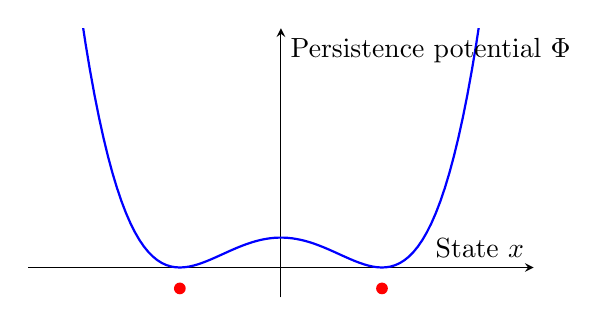
\begin{tikzpicture}
\begin{axis}[
  width=8cm, height=5cm,
  xlabel={State $x$}, ylabel={Persistence potential $\Phi$},
  axis lines=middle,
  ymin=-1, ymax=8,
  xmin=-2.5, xmax=2.5,
  ticks=none
]
\addplot[domain=-2.2:2.2, samples=100, thick, blue] {x^4 - 2*x^2 + 1};
\node at (axis cs: 1,-0.7) [circle, fill=red, inner sep=1.5pt] {};
\node at (axis cs: -1,-0.7) [circle, fill=red, inner sep=1.5pt] {};
\node[below] at (axis cs: 1,-1) {\footnotesize Attractor};
\node[below] at (axis cs: -1,-1) {\footnotesize Attractor};
\end{axis}
\end{tikzpicture}
\caption{Persistence-potential landscape with attractors stabilizing cognitive states, $\Phi(x) = x^4 - 2x^2 + 1$.}
\label{fig:attractor}
\end{figure}

\subsection{Analogies to Biological Processes}

\begin{table}[h]
\centering
\begin{tabular}{ll}
\toprule
\textbf{Biological} & \textbf{Cognitive} \\
\midrule
Cell regeneration & Memory reconsolidation \\
Enzyme repair & Conceptual re-weighting \\
Persistence-potential reduction & Noise filtering \\
\bottomrule
\end{tabular}
\caption{Parallels between biological and cognitive repair processes.}
\label{tab:analogies}
\end{table}

These parallels highlight a shared repair logic across physical and informational longevity, provided the parallel is read as correlational rather than as an unargued identity claim between the two columns.

\subsection{Three Kinds of Recursion}

The architecture developed in this section now has three mutually reinforcing, but conceptually distinct, kinds of recursion rather than one. The Hepastitium of Sections~\ref{sec:hepastitium} supplies recursive physical repair. The allostatic and epistemic machinery of Section~\ref{sec:allostasis} supplies recursive interpretation---revising what a measurement is taken to mean in light of accumulated, and sometimes rejected, evidence. This section's frame-relative treatment of consciousness supplies a third: recursive observer dependence, in which what counts as a phenomenal fact is itself indexed to which cognitive frame is doing the observing. Distinguishing these three registers, rather than treating them as restatements of one underlying idea, is what allows the essay's governing thesis to be stated with three separate clauses rather than one undifferentiated slogan:
\begin{equation}
\boxed{
\begin{aligned}
\text{Somatic longevity} &: \quad \text{repair without loss of the persistence attractor}, \\
\text{Cognitive longevity} &: \quad \text{transformation without loss of frame continuity}, \\
\text{Epistemic longevity} &: \quad \text{revision without collapse into irreversible interpretation}.
\end{aligned}}
\label{eq:three-longevities}
\end{equation}
The Hepastitium is, on this reading, not merely a machine that keeps replacing damaged parts. Its deepest engineering and philosophical problem is deciding what must remain invariant under Equation~\eqref{eq:frame-transformation} while everything else---tissue, morphology, and even the categories under which its own measurements are interpreted---is permitted to change.

\section{Distributed Longevity Across a Lineage}
\label{sec:lineage}

The preceding sections treat longevity as a property an individual organism, institution, or mind either sustains or fails to sustain. But the three-part decomposition of Equation~\eqref{eq:longevity-decomposition} suggests a further possibility: that an individual's own repair capacity, epistemic revisability, and continuation diversity need not all be maximized within that single individual. Some of the burden can be, and empirically is, redistributed across a lineage.

The classical grandparent hypothesis in evolutionary biology holds that post-reproductive longevity persists because older individuals increase the fitness of their descendants' lineage rather than continuing to invest in their own direct reproduction. In the vocabulary of this essay, this is a reallocation across the three terms of Equation~\eqref{eq:longevity-decomposition}: an aging individual's own somatic repair capacity is, on average, declining, but their contribution to the lineage's \emph{epistemic revisability} and \emph{continuation diversity} --- accumulated knowledge, care, and the preservation of alternatives the younger generation has not yet had reason to consider --- need not decline at the same rate, and may even increase. This is exactly the pattern the essay's account of civilizations as distributed reconstruction predicts at a smaller scale: no single generation carries the entirety of a lineage's reconstructive capacity, yet the lineage persists because that capacity is distributed \cite{flyxion2026persistence}.

A related observation concerns cognitive change in aging itself. Reduced prefrontal top-down inhibition and increased variability in neural activity in older adults are often read purely as decline. An alternative reading, consistent with the epistemic-revisability term of Equation~\eqref{eq:longevity-decomposition}, is that a widened, less rigidly filtered search over interpretations is functionally similar to raising the effective temperature in a simulated-annealing search: it trades some precision in any single repair decision for a broader exploration of the interpretation space, which is exactly what prevents the recursive-overfitting hazard identified in Section~\ref{sec:allostasis} from calcifying across an entire lineage's accumulated knowledge. On this reading, elders are not simply individuals whose repair capacity has declined; at the level of the lineage's combined semantic microscope, they are a source of the deliberately retained counterfactuals and rejected interpretations that Section~\ref{sec:allostasis} identified as necessary to prevent recursive overfitting.

This does not license any triumphalist reading of aging, and the essay does not intend one. The claim is narrower and more structural: the three-part decomposition of longevity developed for a single organism has a natural extension to a lineage, in which the terms need not be co-located in any one individual, and in which an individual's declining somatic repair capacity is not the whole of what determines the lineage's own longevity in the sense of Equation~\eqref{eq:longevity-condition}.

\section{Philosophical Implications}

The framework developed in this essay redefines persistence as indefinite renewal through recoverable distinction, resonating with Ortega y Gasset's vital reason and Spinoza's conatus \cite{ortegaygasset1930, spinoza1677}. The Hepastitium's etymology---\emph{hepar} (regeneration) and \emph{stitium} (structure)---mirrors this cosmological point at a smaller scale: every persisting system has a ``liver,'' an interface where damage is repaired into continued recoverability. Longevity is not immortality but the maintained sufficiency of reconstruction against transformation --- a special case of the broader Persistence Principle that whatever can exist, be known, or be experienced must first possess sufficient persistence to remain reconstructible across admissible transformations \cite{flyxion2026persistence}.

\section{Empirical Validation}
\label{sec:empirical}

The framework developed in this essay yields specific, falsifiable predictions across computational, biological, and cognitive domains. Each prediction derives from measurable persistence dynamics and can be expressed as a test of the longevity condition, Equation~\eqref{eq:longevity-condition}. Validation therefore requires observing whether real systems maintain sufficient repair against transformation under controlled perturbation.

\subsection{Simulation Validation}

Physiome, introduced in Section~\ref{sec:physiome} as the measurement and modeling layer for this essay's ontology, offers the most immediate route to empirical exploration, since it already implements the admissibility-and-repair framework of Section~\ref{sec:persistence} across eleven coupled organ systems. Empirical tests consist of measuring the aggregate persistence potential across simulated organ systems under injected perturbation --- infection, hemorrhage, metabolic stress --- and verifying that the simulated organism's repair operators satisfy Equation~\eqref{eq:longevity-condition} within the parameter regimes the model already covers. Because Physiome's homeostatic corrections are implemented as explicit repair operators rather than fixed differential equations, ablating a specific repair operator and observing the resulting drift in persistence potential provides a direct, already-runnable test of the closure and composition claims of Section~\ref{sec:persistence}. More specifically, the recoverable-region contraction of Equation~\eqref{eq:recoverable-contraction} is directly testable in this environment: repeatedly perturbing a simulated organ system by the same nominal insult at different points in a long-running simulation and measuring the time and residual deficit required to return to the admissible set $\mathcal{A}$ gives a concrete, already-computable estimate of $\mathcal{R}_t$'s trajectory, without waiting for any biological experiment.

\subsection{Biomedical Validation}

Biological systems permit direct testing of the framework's central hypothesis. The Hepastitium predicts that continuous microscopic repair should correlate with measurable reductions in persistence potential and improvements in structural recoverability.

\begin{enumerate}[leftmargin=*, label=(\alph*)]
\item \textbf{Reconstruction Error Rate:} Measure the practical analogue of $P(d,T)$ in cultured tissues using microcalorimetry or flux-balance metabolic analysis, tracking how reliably a specific functional distinction (a marker of tissue state) can be recovered after a controlled perturbation. The theory predicts that successful hepastitial interventions lower this reconstruction error while maintaining total energy throughput, indicating increased repair efficiency rather than energy suppression.

\item \textbf{Mitochondrial Order Parameter:} Using super-resolution fluorescence or cryo-electron tomography, quantify mitochondrial cristae organization and membrane potential variability as a proxy for the persistence potential of a specific structural distinction. The framework predicts that hepatic repair processes increase structural coherence---reflected by higher order parameters and lower estimated $\Phi$.

\item \textbf{In Situ Reconstruction Imaging:} Low-dose phase-contrast or terahertz tomography can generate voxelwise persistence-potential maps of tissues. Real-time observation of localized $\Phi$ reduction following micro-intervention would constitute direct validation of Equation~\eqref{eq:repair-operator}.
\end{enumerate}

\subsection{Cognitive Validation}

At the cognitive scale, the framework predicts that conscious stability arises from the maintenance of a self-reconstruction process rather than from any single fixed neural state. Empirical verification requires correlating measures of neural reconstructive capacity with subjective continuity and attentional coherence.

\begin{itemize}[leftmargin=*]
\item \textbf{Neurodynamic Reconstruction Capacity:} Compute multiscale entropy (MSE) or permutation entropy of EEG or fMRI time series, and separately estimate how reliably a given cognitive distinction can be recovered from partial or noisy neural data. The framework predicts a regime of intermediate signal entropy corresponding to maximal reconstructive capacity, rather than either extreme.

\item \textbf{Frame-Coherence Index:} Define an index analogous to $\Phi_c = 1 - \mathrm{Var}(d_i)/\langle d_i \rangle$, where $d_i$ represents regional functional distinctions inferred from neural activation. High $\Phi_c$ indicates coherent self-reconstruction across distributed regions---an empirical correlate of stable conscious presence, in the sense of Section~\ref{sec:cognitive}, without claiming that the index \emph{is} consciousness.

\item \textbf{Repair Deficit Score:} Directly estimate the repair deficit of a cognitive distinction under a controlled perturbation --- e.g. sleep deprivation, a working-memory load, or a pharmacological probe --- as $\delta_R(d,T) = \inf_\rho d_P(\rho(T^*d), d)$ \cite{flyxion2026persistence}. Positive and growing deficits under repeated perturbation would indicate declining cognitive reconstructive capacity; near-zero deficits indicate regenerative, high-reserve states.
\end{itemize}

\subsection{Integrative Metrics}

Together, these experiments motivate a unified set of persistence-derived longevity metrics: a Frame-Coherence Index quantifying self-reconstruction alignment across distributed regions; a Repair Deficit Score measuring the gap between damage and successful reconstruction; and a Persistence Gradient Persistence measure tracking how long local recoverability remains stable under perturbation, as a predictor of regenerative potential.

Across domains, the framework predicts that systems satisfying Equation~\eqref{eq:longevity-condition} will exhibit maximal durability, adaptability, and coherence. Empirical validation therefore converges on a single criterion: whether a system---biological, cognitive, or simulated---can keep its repair operators sufficient against the transformations degrading it, without exhausting the diversity of continuations available to it.

\section{Conclusion}

Persistence is the capacity to keep repair sufficient against transformation, at whatever scale one applies the criterion. This essay has unified biology (the Hepastitium, and its working precursor Physiome), architecture (xylomorphic cities as distributed reconstruction systems), epistemics (the semantic microscope, disciplined by an explicit admission pipeline), cognition (frame continuity under self-reconstruction), and the lineage (distributed longevity across generations) under the single formal apparatus of recoverable distinction developed in Section~\ref{sec:persistence}, rather than under a field-theoretic picture specific to any one substrate. Future directions include the completion of Physiome's remaining subsystems, empirical prototypes of Hepastitium-style tomographic relays, and further development of the ethical framework for hepatic governance sketched in Section~\ref{sec:ethics}.

One further question this essay does not attempt to formalize: when does cumulative repair change the organism's own regime of description, rather than merely repairing it within an unchanged one? A scar, a regenerated liver lobe, a prosthesis, a transplanted organ, extensive cellular replacement, and hypothetical whole-body rejuvenation form a progression in which \emph{repair within a regime} and \emph{transition to another regime} become progressively harder to distinguish. A scale-sensitive mereology capable of marking such regime boundaries explicitly, of the kind developed elsewhere in the author's work on layered part-whole description, may eventually supply the vocabulary this essay currently lacks for that distinction; it is not attempted here.

\appendix

\section{An Optional Field-Theoretic Restatement (RSVP)}
\label{app:rsvp}

Readers familiar with the author's earlier Relativistic Scalar-Vector Plenum (RSVP) field theory may find it useful to see the repair-theoretic account above restated in that vocabulary. Nothing in the main text depends on this appendix.

RSVP models a persisting system through three coupled fields: scalar capacity $\Phi_{\mathrm{RSVP}}$, representing informational or functional capacity; vector flow $\mathbf{v}$, denoting directed transport of resources or agents; and entropy field $S$, quantifying disorder. Their evolution is governed by
\begin{align}
\frac{d\Phi_{\mathrm{RSVP}}}{dt} &= -\nabla \cdot (\mathbf{v}\Phi_{\mathrm{RSVP}}) + \lambda(S_c - S) + \sum_k \alpha_k \delta\Phi_k, \\
\frac{d\mathbf{v}}{dt} &= -\nabla\Phi_{\mathrm{RSVP}} - \beta(\mathbf{v}\cdot\nabla)\mathbf{v} + \xi \nabla S, \\
\frac{dS}{dt} &= \kappa \nabla^2 S - \sum_k \gamma_k \Delta S_k,
\end{align}
with a hepatic operator $\mathcal{H}[\Phi_{\mathrm{RSVP}}, \mathbf{v}, S]$ enforcing the persistence criterion
\begin{equation}
\langle \mathcal{H} \rangle_\Omega \le 0.
\label{eq:rsvp-criterion}
\end{equation}
The correspondence with the main text is direct: $\Phi_{\mathrm{RSVP}}$ plays the role of an inverse persistence potential (high capacity corresponds to low $\Phi(d)$ in the main text's notation), $S$ plays the role of aggregate unrepaired damage, and $\mathcal{H}$ plays the role of the aggregate repair operator whose sufficiency Equation~\eqref{eq:longevity-condition} demands. Equation~\eqref{eq:rsvp-criterion} and Equation~\eqref{eq:longevity-condition} express the same underlying requirement --- that repair keep pace with transformation --- in field-theoretic and reconstruction-theoretic vocabularies respectively. Readers who prefer partial differential equations to structured domains may use whichever restatement they find more tractable; the essay's substantive claims are stated, and should be evaluated, in the vocabulary of Section~\ref{sec:persistence}.

\section{Semantic Microscope Pseudocode}

\begin{lstlisting}[language=JavaScriptRSVP, caption={Semantic microscope query traversal.}, label={lst:semantic-microscope}]
function semanticMicroscope(G, query):
    results = []
    for node in G.nodes:
        if matches(query, node):
            results.append(traceCausalPath(G, node))
    return results
\end{lstlisting}

\section{Glossary}

\begin{description}[leftmargin=2.4cm, style=nextline]
\item[Structured Domain] A quadruple $\mathfrak{D} = (X, \mathcal{T}, \mathcal{D}, \mathcal{R})$: a state space, a family of transformations, a family of distinctions, and a family of reconstruction operators. The basic unit of analysis throughout this essay.

\item[Recoverable Distinction] A distinction $d$ such that $d \circ R \circ T = d$ for some admissible reconstruction operator $R$ and transformation $T$. Strictly generalizes classical invariance.

\item[Persistence Potential $\Phi(d)$] The expected reconstruction error a distinction would incur under the transformations it is likely to face. Low $\Phi$ indicates robustness; high $\Phi$ indicates fragility.

\item[Repair Operator] A map $\rho : \mathcal{D} \to \mathcal{D}$ satisfying $\Phi(\rho(d)) \le \Phi(d)$. Repair operators compose, and their composition is itself a repair operator.

\item[Persistence Attractor] An equivalence class of states toward which repeated reconstruction converges. The formal basis for treating identity --- of an organism, an institution, or a self --- as a matter of reconstructive continuity rather than material constancy.

\item[Longevity Condition] The requirement, Equation~\eqref{eq:longevity-condition}, that an organism's repair regime not let persistence potential drift upward on average across cycles of damage and repair.

\item[Hepastitium] Contraction of \emph{hepatostitium} (Greek \emph{hepar}, ``liver''; Latin \emph{stitium}, ``standing-place''). The proposed endogenous tissue-sampling and microsurgical relay network implementing distributed repair operators across the whole body.

\item[Physiome] The author's working Rust-based whole-body physiology simulator, implementing eleven organ systems via admissibility and repair operators. The present-day computational instantiation of the Hepastitium's diagnostic and homeostatic half.

\item[Record-Recognize-Interpret-Admit-Intervene-Verify (RRAIV)] The pipeline, Equation~\eqref{eq:rraiv}, disciplining when a detected deviation is permitted to trigger a repair intervention.

\item[Cognitive Frame of Reference] The first-person perspective from which self-reconstruction, in the persistence-theoretic sense, occurs; distinct from, but complementary to, the persistence-attractor account of the self.

\item[Repair Deficit] The residual discrepancy remaining after optimal available repair, $\delta_R(d,T) = \inf_\rho d_P(\rho(T^*d), d)$. Vanishes exactly when the distinction is perfectly recoverable.
\end{description}

\begin{thebibliography}{9}

\bibitem{prigogine1977}
Prigogine, I. \emph{Time, Structure and Fluctuations}. 1977.

\bibitem{schrodinger1944}
Schr\"odinger, E. \emph{What is Life?} 1944.

\bibitem{friston2010}
Friston, K. The Free-Energy Principle: A Unified Brain Theory? \emph{Nature Reviews Neuroscience}, 11(2):127--138, 2010.

\bibitem{ortegaygasset1930}
Ortega y Gasset, J. \emph{The Revolt of the Masses}. 1930.

\bibitem{spinoza1677}
Spinoza, B. \emph{Ethics}. 1677.

\bibitem{lahavneemeh2022}
Lahav, N. and Neemeh, Z. A. A Relativistic Theory of Consciousness. \emph{Frontiers in Psychology}, 12:704270, 2022.

\bibitem{barrettmiller2026longevity}
Barrett, L. F. and Miller, E. K. Categorization is `baked' into the brain. \emph{Nature Reviews Neuroscience}, 27:435--456, 2026.

\bibitem{sterling2012}
Sterling, P. Allostasis: A model of predictive regulation. \emph{Physiology \& Behavior}, 106(1):5--15, 2012.

\bibitem{flyxion2026persistence}
Flyxion. \emph{Persistence Before Truth: Recoverable Distinction as the Condition of Reference, Explanation, and Knowledge}. 2026.

\bibitem{flyxion2026worldhood}
Flyxion. \emph{Irreversibility and Worldhood as Consciousness}. 2026.

\end{thebibliography}

\end{document}

